\setcounter{chapter}{11}
\chapter{Texture}
\begin{compactdesc}
\item[\lp{Key issue}] Representing texture\\
	\begin{enumerate*}[label=\protect\circled{\arabic*},itemjoin=]
		\item Texture analysis/segmentation $\to$ representing texture\\
		\item Texture synthesis: Useful, also gives some insight into quality of representation\\
		\item Shape from texture
	\end{enumerate*}
	Computer graphics: texture mapping
\item[\lp{General}]\hfill \\
	\begin{itemize*}[label=\colorbullet]
		\item Textures are made up of quite stylised subelements, repeated in meaningful ways.\\
		\item Representation: Find the subelements, and represent their statistics.\\
		\item Subelements: Normalized correlation, apply filters.\\
		\item Filters: Spots and oriented bars at a variety of different scales (by experience), details probably don't matter\\
		\item Statistics: Within reason, the more the merrier. At least, mean and standard deviation. Better, various conditional histograms.
	\end{itemize*}
\item[\lp{Oriented pyramids}] Laplacian pyramid is orientation independent. Apply an oriented filter to determine orientations at each leayer. By clever filter design, we can simplify synthesis. This represents image information at a particular scale and orientation.
	\item[\lp{Final texture representation}] \hfill\\
		\begin{enumerate*}[label=\protect\circled{\arabic*},itemjoin=]\hfill\\
			\item Form an oriented pyramid (or equivalent set of responses to filters at different scales and orientations)\\
			\item Square the output\\
			\item Take statistics of responses\\
				\begin{enumerate*}[label=\quad\protect\circled{\alph*},itemjoin=]
					\item e.g. mean of each filter output (are there lots of spots)\\
					\item std of each filter output\\
					\item mean of one scale conditioned on other scale having a particular range of values (e.g. are the spots in straight rows?)
				\end{enumerate*}
		\end{enumerate*}
	\item[\lp{Texture synthesis}] \hfill\\
		\begin{enumerate*}[label=\protect\circled{\arabic*},itemjoin=]
			\item Use image as a source of probability model\\
			\item Choose pixel values by matching neighbourhood, then filling in\\
			\item Matching process: Look at pixel differences, count only sythesized pixels
		\end{enumerate*}
\section{Histogram}
	\item[\lp{Principle}] \hfill\\
		\begin{enumerate*}[label=\protect\circled{\arabic*},itemjoin=]
			\item Intensity probability distribution\\
			\item Captures global brightness information in a compact, but incomplete way\\
			\item Doesn't capture spatial relationships
		\end{enumerate*}
	\item[\lp{Co-occurrence matrix}] Is a matrix or distribution that is defined over an image to be the distribution of co-occurring values at a given offset. Mathematically, a co-occurence matrix $C$ is defined over an $n\times m$ image $I$, parametrized by an offset $\left( \Delta x,\Delta y \right)$ as:
		\begin{gather*}
			C_{\Delta x,\Delta y}(i,j)={\scriptstyle\sum\limits_{p=1}^{n}}{\scriptstyle\sum\limits_{q=1}^{m}}
			\begin{cases}
				1&\text{if }\spadesuit,\\
				0&\text{else}.
			\end{cases}
		\end{gather*}
		$\spadesuit$: $I(p,q)=i$,  $I(p+\Delta x,q+\Delta y)=j$. \\
		For an image with grey tones
		\begin{gather*}
			\!\left(\!\begin{smallmatrix}
				0&0&1&1\\
				0&0&1&1\\
				0&2&2&2\\
				2&2&3&3
			\end{smallmatrix}\!\right)\!
		\end{gather*}
		Compute
		\begin{gather*}
			\begin{array}[]{*{5}{>{\scriptstyle\hskip-1ex}c<{\hskip-1ex}}}
				\multicolumn{1}{c}{}&0&1&2&3\\
				\toprule
				0&\#(0,0)&\#(0,1)&\#(0,2)&\#(0,3)\\
				1&\#(1,0)&\#(1,1)&\#(1,2)&\#(1,3)\\
				2&\#(2,0)&\#(2,1)&\#(2,2)&\#(2,3)\\
				3&\#(3,0)&\#(3,1)&\#(3,2)&\#(3,3)
			\end{array}
		\end{gather*}
		\begin{align*}
\SI{0}{\degree}:&&
	P_{\text{horizontal}}&=
			\!\left(\!\begin{smallmatrix}
				4&2&1&0\\
				2&4&0&0\\
				1&0&6&1\\
				0&0&1&2
			\end{smallmatrix}\!\right)\!\\
			\SI{45}{\degree}:&&	P_{\text{right diag.}}&=
			\!\left(\!\begin{smallmatrix}
				4&1&0&0\\
				1&2&2&0\\
				0&2&4&1\\
				0&0&1&0
			\end{smallmatrix}\!\right)\!
		\end{align*}
\section{Texture synthesis}
	\item[\lp{Goal}] Texture synthesis algorithms are intended to create an \emph{output image} that meets the following requirements:\\
		\begin{enumerate*}[label=\protect\circled{\arabic*},itemjoin=]
			\item The output should have the size given by the user.\\
			\item The output should be as similar as possible to the sample.\\
			\item The output should not have visible artifacts such as seams, blocks and misfitting edges.\\
			\item The output should not repeat, i. e. the same structures in the output image should not appear multiple places.\\
		\end{enumerate*}
Like most algorithms, texture synthesis should be efficient in computation time and in memory use.
\subsection{Methods}
\item[\lp{View-dependent texture synthesis}] One can create textures viewed from different angles.
\item[\lp{Clique Type Selection}]\hfill\\
	\begin{enumerate*}[label=\lp{step \arabic*},itemjoin=]
		\item  Collect the complete 2nd-order statistics for the example texture, i.e., the intensity difference distributions of all clique types up to a maximum length.  After this step the example texture is no longer needed.\\
		\item Generate an image filled with independent noise with values uniformly distributed in the range of the example texture. This noise image serves as the initial synthesized texture, to be refined in subsequent steps.\\
		\item Collect the pairwise statistics of all clique types (up to the same maximal length) for the current synthesized image (initially noise).\\
		\item For each clique type, compare the difference distributions of the example texture and the synthesized texture by calculating the Euclidean distance.\\
		\item Select the clique type with the maximal distance. If this distance is less than some threshold go to step 8 - the end of the algorithm. Otherwise, add the clique type to the (initially empty) neighborhood system and its difference distribution to the (initially empty) parameter set.\\
		\item Synthesize a new texture using the updated neighborhood system and parameter set. The texture should have the prescribed statistics for all clique types in the neighborhood system.\\
		\item Go to step 3.\\
		\item End of the algorithm.\\
	\end{enumerate*}
	The distribution distances that are compared between clique types in step 4 are weighted with the number of cliques. This should prevent unstable statistical behavior when there are only few cliques (typical for lang clique types.)
	\item[\lp{Tiling}] The simplest way to generate a large image from a sample image is to tile it. This means multiple copies of the sample are simply copied and pasted side by side. The result is rarely satisfactory. Except in rare cases, there will be the seams in between the tiles and the image will be highly repetitive.
	\item[\lp{Stochastic texture synthesis}] Stochastic texture synthesis methods produce an image by randomly choosing colour values for each pixel, only influenced by basic parameters like minimum brightness, average colour or maximum contrast. These algorithms perform well with stochastic textures only, otherwise they produce completely unsatisfactory results as they ignore any kind of structure within the sample image.
	\item[\lp{Single purpose structured }] 
	\item[\lp{texture synthesis}]
		Algorithms of that family use a fixed procedure to create an output image, i. e. they are limited to a single kind of structured texture. Thus, these algorithms can both only be applied to structured textures and only to textures with a very similar structure. For example, a single purpose algorithm could produce high quality texture images of stonewalls; yet, it is very unlikely that the algorithm will produce any viable output if given a sample image that shows pebbles.
	\item[\lp{Chaos mosaic}] This method, proposed by the Microsoft group for internet graphics, is a refined version of tiling and performs the following three steps:\\
		\begin{enumerate*}[label=\protect\circled{\arabic*},itemjoin=]
			\item The output image is filled completely by tiling. The result is a repetitive image with visible seams.\\
			\item Randomly selected parts of random size of the sample are copied and pasted randomly onto the output image. The result is a rather non-repetitive image with visible seams.\\
			\item The output image is filtered to smooth edges.\\
		\end{enumerate*}
		The result is an acceptable texture image, which is not too repetitive and does not contain too many artifacts. Still, this method is unsatisfactory because the smoothing in step 3 makes the output image look blurred.
	\item[\lp{Pixel-based texture synthesis}] 
		These methods, such as "Texture synthesis via a noncausal nonparametric multiscale Markov random field." Paget and Longstaff, IEEE Trans. on Image Processing, 1998, "Texture Synthesis by Non-parametric Sampling." Efros and Leung, ICCV, 1999,
		\begin{itemize*}[label=\colorbullet]
			\item Assuming Markov property, compute $P(p|N(p))$. Building explicit probability tables infeasible. Instead, let's search the input image for all similar neighborhoods - that's our histogram for $p$. to synthesize $p$, just pick one match at random.
		\end{itemize*}
		"Fast Texture Synthesis using Tree-structured Vector Quantization" Wei and Levoy SIGGRAPH 2000 and "Image Analogies" Hertzmann et al. SIGGRAPH 2001. are some of the simplest and most successful general texture synthesis algorithms. They typically synthesize a texture in scan-line order by finding and copying pixels with the most similar local neighborhood as the synthetic texture. These methods are very useful for image completion. They can be constrained, as in image analogies, to perform many interesting tasks. They are typically accelerated with some form of Approximate Nearest Neighbor method since the exhaustive search for the best pixel is somewhat slow. The synthesis can also be performed in multiresolution, such as "Texture synthesis via a noncausal nonparametric multiscale Markov random field." Paget and Longstaff, IEEE Trans. on Image Processing, 1998.
	\item[\lp{Patch-based texture synthesis}] Patch-based texture synthesis creates a new texture by copying and stitching together textures at various offsets, similar to the use of the clone tool to manually synthesize a texture. "Image Quilting." Efros and Freeman. SIGGRAPH 2001 and "Graphcut Textures: Image and Video Synthesis Using Graph Cuts." Kwatra et al. SIGGRAPH 2003 are the best known patch-based texture synthesis algorithms. These algorithms tend to be more effective and faster than pixel-based texture synthesis methods.
	\item[\lp{Chemistry based}] Realistic textures can be generated by simulations of complex chemical reactions within fluids, namely Reaction-diffusion systems. It is believed that these systems show behaviors which are qualitatively equivalent to real processes (Morphogenesis) found in the nature, such as animal markings (shells, fish, wild cats\ldots).
	\item[\lp{Efros \& Leung ' 99 extended}] Observation: neighbor pixels are highly correlated. Idea: Unit of synthesis is block
		\begin{itemize*}[label=\colorbullet]
			\item Exactly the same but now we want $P(B|N(B))$.\\
			\item Much faster: Synthesize all pixes in a block at once\\
			\item Not the same as multi-scale\\
		\end{itemize*}
		\def\rsize{0.7}
		\def\hrsize{0.5*\rsize}
		\def\phsize{1.5*\rsize}
		\def\lwidth{1}
		\def\textpos{1.8}
		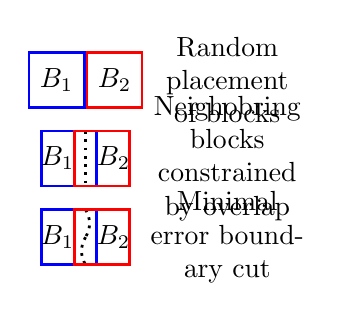
\begin{tikzpicture}[myrec/.style=inner sep=0pt,rectangle,draw,line width=\lwidth pt,minimum width=\rsize cm,minimum height=0.7cm,redrec/.style={draw=red,myrec},bluerec/.style={draw=blue,myrec}]
			\node[bluerec] (b11) at (-\hrsize cm-0.5*\lwidth pt,0) {$B_1$};
			\node[redrec] (b21) at (\hrsize cm+0.5*\lwidth pt,0) {$B_2$};
			\node[text width=2cm,align=center] (t1) at (\textpos,0) {Random placement of blocks};
			\begin{scope}[shift={(0,-1)}]
				\draw[dotted] (0,\hrsize) -- (0,-\hrsize);
				\node[bluerec] (b12) at (-0.6*\hrsize cm,0) {$\!\!\!\!\!B_1$};
				\node[redrec] (b22) at (0.6*\hrsize cm,0) {$B_2\!\!\!\!\!$};
				\node[text width=2cm,align=center] (t2) at (\textpos,0) {Neighobring blocks constrained by overlap};
			\end{scope}
			\begin{scope}[shift={(0,-2)}]
				\path[draw,dotted] (0,\hrsize) to[bend left] node{} (0,0);
				\path[draw,dotted] (0,0) to[bend right] node{} (0,-\hrsize);
				\node[bluerec] (b13) at (-0.6*\hrsize cm,0) {$\!\!\!\!\!B_1$};
				\node[redrec] (b23) at (0.6*\hrsize cm,0) {$B_2\!\!\!\!\!$};
				\node[text width=2cm,align=center] (t3) at (\textpos,0) {Minimal error boundary cut};
			\end{scope}
		\end{tikzpicture}
		Algorithm
		\begin{enumerate*}[label=\protect\circled{\arabic*},itemjoin=]
			\item Pick size of block and size of overlap\\
			\item Synthesize blocks in raster order\\
			\item Search input texture for bolck that satisfies overlap constraints (above and left)\\
			\item Paste new block into resulting texture. Use dynamic programming to compute minimal error boundary cut
		\end{enumerate*}
		\section{Texture Transfer} Take the texture from one object and ``paint'' it onto another object. This requires spearating texture and shape. That's hard, but we can cheat. Assume we can capture shape by baundary and rough shading. Then, just add another constraint when sampling: similarity to underlying image at that spot.
	\item[\lp{Shape from textures}] Possibility to recover normals both for deterministic and probabilistic textures.
\end{compactdesc}
